\documentclass{beamer}
\usetheme{default}
\usepackage{tikz}
\usetikzlibrary{positioning}
\tikzset{main node/.style={circle,fill=teal!60,draw,minimum size=1cm,inner sep=0pt},
}

\title{CS 584: Spatial Computing Assignment 7: Spatial Networks}
\author{Mitchell Scott}
\institute{Emory University}
\begin{document}
\begin{frame}[plain]
    \maketitle
\end{frame}
\begin{frame}[allowframebreaks]{Assignment 7-1}
	\begin{center}
	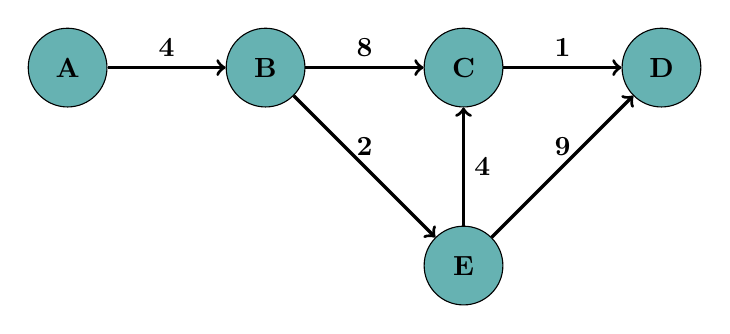
\begin{tikzpicture}
		\node[main node] (A) {\textbf{A}};
		\node[main node] (B) [right =1.5cm of A]  {\textbf{B}};
		\node[main node] (C) [right = 1.5cm of B] {\textbf{C}};
		\node[main node] (D) [right = 1.5cm of C] {\textbf{D}};
		\node[main node] (E) [below = 1.5cm of C] {\textbf{E}};
		
		\path[draw,very thick,->]
		(A) edge node[above] {\textbf{4}} (B)
		(B) edge node[above] {\textbf{8}} (C)
		(B) edge node[above] {\textbf{2}} (E)
		(C) edge node[above] {\textbf{1}} (D)
		(E) edge node[right] {\textbf{4}} (C)
		(E) edge node[above] {\textbf{9}} (D);
		
	\end{tikzpicture}
	\end{center}
	\begin{enumerate}
		\item {\bf Is this network directed or undirected? Explain your answers!}
		\begin{solution}
			This network is \textbf{directed} since it is possible to get from \textbf{A} to \textbf{B}, but impossible to get from \textbf{B} to \textbf{A}. The arrow with one direction indicates that the edge is uni-directional, so a directed graph.
		\end{solution}
		\item {\bf Which nodes are adjacent to Node B?}
		\begin{solution}
			Since we are in a directed graph, the definition for \textbf{adjacent} is two vertices $v_1, v_2$ are adjacent if $(v_1,v_2)\in E$\footnote{where $E$ is the edge set and \textbf{E} is the node.} OR $(v_2,v_1)\in E$. This means \textbf{A} is adjacent to \textbf{B} since (\textbf{A},\textbf{B})$\in E$. Similarly, the vertices that \textbf{B} points to are adjacent, which are \textbf{C}, \textbf{D} since (\textbf{B},\textbf{C})$\in E$, (\textbf{B},\textbf{E})$\in E$. \\
			
			Thus the set of all nodes adjacent to \textbf{B} are \{\textbf{A}, \textbf{C}, \textbf{E}\}.
		\end{solution}
		\item {\bf What is the degree of Node C?}
		\begin{solution}
			Since the definition of \textbf{degree} is the `` number of outgoing edges, then $\deg$ \textbf{C} = 1, as it has two incoming edges but only one outgoing edge.
		\end{solution}
		\item {\bf In class we talked about representing a network as a \emph{labelled} adjacency matrix (or cost matrix). Provide the labelled adjacency matrix (cost matrix) for the network above.}
		\begin{solution}
		\begin{table}
			\centering
				\begin{tabular}{c|ccccc}
				& \textbf{A} & \textbf{B} & \textbf{C} & \textbf{D}& \textbf{E}\\
				\hline
				\textbf{A} & 0 &4 &$\infty$ &$\infty$ &$\infty$ \\
				\textbf{B} &  $\infty$& 0&8 &$\infty$ & 2\\
				\textbf{C} &$\infty$  &$\infty$ & 0& 1& $\infty$\\
				\textbf{D} &$\infty$  &$\infty$ & $\infty$&0& $\infty$\\
				\textbf{E} &$\infty$  &$\infty$ &4 & 9& 0\\
			\end{tabular}
			\label{tab:costmat}
			\caption{Cost Matrix where staying at the same node is 0 cost, and non existing edges are denoted by `$\infty$'. }
		\end{table}
		\end{solution}
	\end{enumerate}
\end{frame}
\begin{frame}[allowframebreaks]{Assignment 7-2}
	\begin{itemize}
		\item at Step 0, we haven't seen anything yet.
	\end{itemize}
	\begin{columns}
		\column{0.7\textwidth}
		\begin{center}
			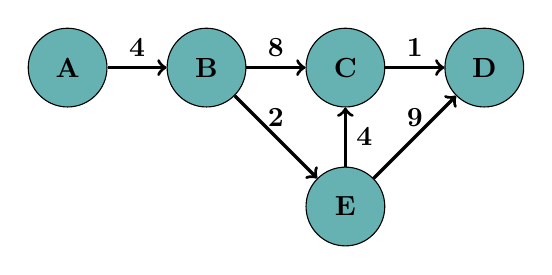
\begin{tikzpicture}
				\node[main node] (A) {\textbf{A}};
				\node[main node] (B) [right =0.75cm of A]  {\textbf{B}};
				\node[main node] (C) [right = 0.75cm of B] {\textbf{C}};
				\node[main node] (D) [right = 0.75cm of C] {\textbf{D}};
				\node[main node] (E) [below = 0.75cm of C] {\textbf{E}};
				
				\path[draw,very thick,->]
				(A) edge node[above] {\textbf{4}} (B)
				(B) edge node[above] {\textbf{8}} (C)
				(B) edge node[above] {\textbf{2}} (E)
				(C) edge node[above] {\textbf{1}} (D)
				(E) edge node[right] {\textbf{4}} (C)
				(E) edge node[above] {\textbf{9}} (D);
				
			\end{tikzpicture}
		\end{center}
		\column{0.3\textwidth}
		\begin{tabular}{rc}
			Node & Dist.\\
			\hline
			\colorbox{lightgray}{\textbf{A}:} & $\infty$\\
			\colorbox{lightgray}{\textbf{B}:} & $\infty$\\
			\colorbox{lightgray}{\textbf{C}:} & $\infty$\\
			\colorbox{lightgray}{\textbf{D}:} & $\infty$\\
			\colorbox{lightgray}{\textbf{E}:} & $\infty$\\
		\end{tabular}
	\end{columns}
		\begin{itemize}
		\item at Step 1, we mark \textbf{A} as green with a distance of 0, and go to \textbf{B} with distance 4.
	\end{itemize}
	\begin{columns}
		\column{0.7\textwidth}
		\begin{center}
			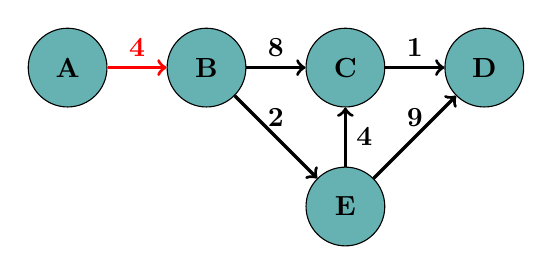
\begin{tikzpicture}
				\node[main node] (A) {\textbf{A}};
				\node[main node] (B) [right =0.75cm of A]  {\textbf{B}};
				\node[main node] (C) [right = 0.75cm of B] {\textbf{C}};
				\node[main node] (D) [right = 0.75cm of C] {\textbf{D}};
				\node[main node] (E) [below = 0.75cm of C] {\textbf{E}};
				
				\path[draw,very thick,->]
				(A) edge[red] node[above] {\textbf{4}} (B)
				(B) edge node[above] {\textbf{8}} (C)
				(B) edge node[above] {\textbf{2}} (E)
				(C) edge node[above] {\textbf{1}} (D)
				(E) edge node[right] {\textbf{4}} (C)
				(E) edge node[above] {\textbf{9}} (D);
				
			\end{tikzpicture}
		\end{center}
		\column{0.3\textwidth}
		\begin{tabular}{rc}
			Node & Dist.\\
			\hline
			\colorbox{green}{\textbf{A}:} &0 \\
			\colorbox{yellow}{\textbf{B}:} & 4\\
			\colorbox{lightgray}{\textbf{C}:} &$\infty$ \\
			\colorbox{lightgray}{\textbf{D}:} & $\infty$\\
			\colorbox{lightgray}{\textbf{E}:} & $\infty$\\
		\end{tabular}
	\end{columns}
		\begin{itemize}
		\item at Step 2, we mark \textbf{B} as green with a distance of 4, and go to \textbf{E} with distance 6.
	\end{itemize}
	\begin{columns}
		\column{0.7\textwidth}
		\begin{center}
			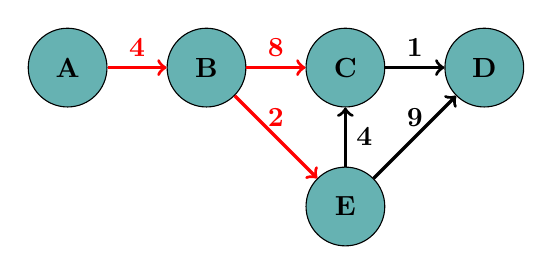
\begin{tikzpicture}
				\node[main node] (A) {\textbf{A}};
				\node[main node] (B) [right =0.75cm of A]  {\textbf{B}};
				\node[main node] (C) [right = 0.75cm of B] {\textbf{C}};
				\node[main node] (D) [right = 0.75cm of C] {\textbf{D}};
				\node[main node] (E) [below = 0.75cm of C] {\textbf{E}};
				
				\path[draw,very thick,->]
				(A) edge[red] node[above] {\textbf{4}} (B)
				(B) edge[red] node[above] {\textbf{8}} (C)
				(B) edge[red] node[above] {\textbf{2}} (E)
				(C) edge node[above] {\textbf{1}} (D)
				(E) edge node[right] {\textbf{4}} (C)
				(E) edge node[above] {\textbf{9}} (D);
				
			\end{tikzpicture}
		\end{center}
		\column{0.3\textwidth}
		\begin{tabular}{rc}
			Node & Dist.\\
			\hline
			\colorbox{green}{\textbf{A}:} &0 \\
			\colorbox{green}{\textbf{B}:} & 4\\
			\colorbox{yellow}{\textbf{C}:} &12 \\
			\colorbox{lightgray}{\textbf{D}:} & $\infty$\\
			\colorbox{yellow}{\textbf{E}:} & 6\\
		\end{tabular}
	\end{columns}
	\begin{itemize}
		\item at Step 3, we mark \textbf{E} as green with a distance of 6, and go to \textbf{C} with ($^\ast$updated) distance 10.
	\end{itemize}
	\begin{columns}
		\column{0.7\textwidth}
		\begin{center}
			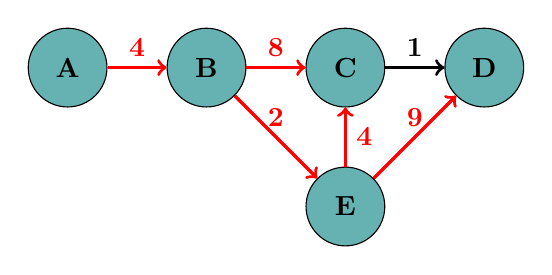
\begin{tikzpicture}
				\node[main node] (A) {\textbf{A}};
				\node[main node] (B) [right =0.75cm of A]  {\textbf{B}};
				\node[main node] (C) [right = 0.75cm of B] {\textbf{C}};
				\node[main node] (D) [right = 0.75cm of C] {\textbf{D}};
				\node[main node] (E) [below = 0.75cm of C] {\textbf{E}};
				
				\path[draw,very thick,->]
				(A) edge[red] node[above] {\textbf{4}} (B)
				(B) edge[red] node[above] {\textbf{8}} (C)
				(B) edge[red] node[above] {\textbf{2}} (E)
				(C) edge node[above] {\textbf{1}} (D)
				(E) edge[red] node[right] {\textbf{4}} (C)
				(E) edge[red] node[above] {\textbf{9}} (D);
				
			\end{tikzpicture}
		\end{center}
		\column{0.3\textwidth}
		\begin{tabular}{rc}
			Node & Dist.\\
			\hline
			\colorbox{green}{\textbf{A}:} &0 \\
			\colorbox{green}{\textbf{B}:} & 4\\
			\colorbox{yellow}{\textbf{C}:} &10$^\ast$ \\
			\colorbox{yellow}{\textbf{D}:} & 15\\
			\colorbox{green}{\textbf{E}:} & 6\\
		\end{tabular}
	\end{columns}
		\begin{itemize}
		\item at Step 4, we mark \textbf{C} as green with a distance of 10, and go to \textbf{D} with ($^\ast$updated) distance 11.
	\end{itemize}
	\begin{columns}
		\column{0.7\textwidth}
		\begin{center}
			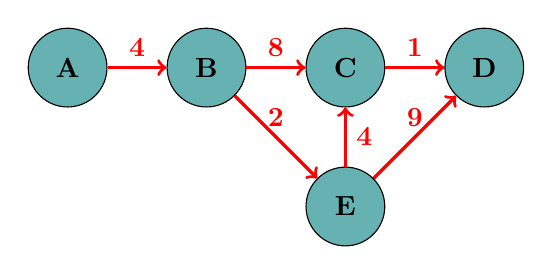
\begin{tikzpicture}
				\node[main node] (A) {\textbf{A}};
				\node[main node] (B) [right =0.75cm of A]  {\textbf{B}};
				\node[main node] (C) [right = 0.75cm of B] {\textbf{C}};
				\node[main node] (D) [right = 0.75cm of C] {\textbf{D}};
				\node[main node] (E) [below = 0.75cm of C] {\textbf{E}};
				
				\path[draw,very thick,->]
				(A) edge[red] node[above] {\textbf{4}} (B)
				(B) edge[red] node[above] {\textbf{8}} (C)
				(B) edge[red] node[above] {\textbf{2}} (E)
				(C) edge[red] node[above] {\textbf{1}} (D)
				(E) edge[red] node[right] {\textbf{4}} (C)
				(E) edge[red] node[above] {\textbf{9}} (D);
				
			\end{tikzpicture}
		\end{center}
		\column{0.3\textwidth}
		\begin{tabular}{rc}
			Node & Dist.\\
			\hline
			\colorbox{green}{\textbf{A}:} &0 \\
			\colorbox{green}{\textbf{B}:} & 4\\
			\colorbox{green}{\textbf{C}:} &10 \\
			\colorbox{yellow}{\textbf{D}:} & 11$^\ast$\\
			\colorbox{green}{\textbf{E}:} & 6\\
		\end{tabular}
	\end{columns}
	\begin{itemize}
		\item at Step 5, we mark \textbf{D} as green with a distance of 11. With no more yellow nodes, we terminate.
	\end{itemize}
	\begin{columns}
		\column{0.7\textwidth}
		\begin{center}
			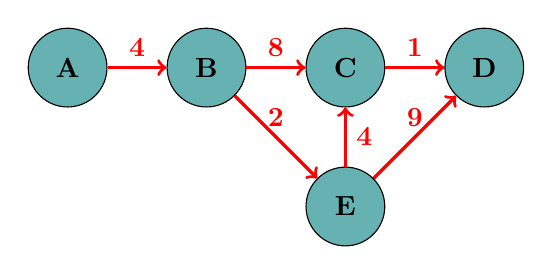
\begin{tikzpicture}
				\node[main node] (A) {\textbf{A}};
				\node[main node] (B) [right =0.75cm of A]  {\textbf{B}};
				\node[main node] (C) [right = 0.75cm of B] {\textbf{C}};
				\node[main node] (D) [right = 0.75cm of C] {\textbf{D}};
				\node[main node] (E) [below = 0.75cm of C] {\textbf{E}};
				
				\path[draw,very thick,->]
				(A) edge[red] node[above] {\textbf{4}} (B)
				(B) edge[red] node[above] {\textbf{8}} (C)
				(B) edge[red] node[above] {\textbf{2}} (E)
				(C) edge[red] node[above] {\textbf{1}} (D)
				(E) edge[red] node[right] {\textbf{4}} (C)
				(E) edge[red] node[above] {\textbf{9}} (D);
				
			\end{tikzpicture}
		\end{center}
		\column{0.3\textwidth}
		\begin{tabular}{rc}
			Node & Dist.\\
			\hline
			\colorbox{green}{\textbf{A}:} &0 \\
			\colorbox{green}{\textbf{B}:} & 4\\
			\colorbox{green}{\textbf{C}:} &10 \\
			\colorbox{green}{\textbf{D}:} & 11\\
			\colorbox{green}{\textbf{E}:} & 6\\
		\end{tabular}
	\end{columns}
	
\end{frame}
\end{document}
